\section*{Глава 3. Неизотермическая фильтрация флюида к несовершенным скважинам.}
\addcontentsline{toc}{section}{Глава 3. Неизотермическая фильтрация флюида к несовершенным скважинам.}

\setcounter{section}{3}
\setcounter{subsection}{0}
\setcounter{equation}{0}

	В данной главе будут описаны виды несовершенств скважины, рассматриваемые в представленной работе.
	Будут описаны методики расчёта дополнительного гидродинамического сопротивления (скин-фактора) применяемые в нефтяной практике.
	Затем будет представлено аналитическое решение простейшей модели неизотермической фильтрации, рассмотрено влияние описаных несовершенств на динамику забойной температуры, метод термозондирования пласта. Будет представлено сравнение расчётов с рассматриваемой аналитикой.

\subsection{Виды несовершенств}
	В ходе бурения, освоения и эксплуатации скважины различные технологические процессы воздействуют на ОЗП.
	В результате её ФЕС меняются.
	Отличие притока скважины от притока, рассчитанного по формуле Дюпюи учитывают, вводя \textit{скин-фактор} $s$:
\begin{equation}
	\label{dupuit}
	Q = \frac{2\pi k h}{\mu B \left(\ln\displaystyle\frac{r_e}{r_w}+s\right)}
\end{equation}

	Понятие скин-фактора достаточно расплывчато, на него списывают любое отличие от выражения \eqref{dupuit}, зачастую не уточняя чем то или иное дополнительно фильтрационное сопротивление (или даже проводимость) вызвано. Предполагается, что скин-фактор аддитивен. В общем виде можно его представить как \cite{mukerdzhi}:
\begin{equation}
	\label{skin_full}
	s = s_d + s_p + s_{pp} + s_{turb} + s_o + s_s + \cdots,
\end{equation}
	где
\begin{itemize}
\item $s_d$ -- скин эф-т вследствие повреждения породы,
\item $s_p$ -- скин эф-т из-за перфорации,
\item $s_{pp}$ -- скин эф-т вследствие частичного проникновения скважины в пласт,
\item $s_{turb}$ -- скин эф-т вследствие турбуленции или скин, зависящий от темпа отбора,
\item $s_{o}$ -- скин-эффект вследствие наклона скважины,
\item $s_{s}$ -- скин-эффект, возникающий вследствие стимуляции, применения различных МУН.
\end{itemize}
	С формальной точки зрения, каждый из перечисленных выше скин-факторов -- упрощение модели фильтрации и её сведение к случаю радиальной притока. В данной работе будут рассмотрены лишь первые три фактора ($s_d$, $s_p$, $s_{pp}$) из перечисленных, обуславливающие несовершенство скважины, в явной математической поставке, без каких-либо упрощений.

\subsubsection{Повреждение ОЗП}
	В процессе бурения скважины происходит загрязнение ОЗП фильтратом бурового раствора.
	В дальнейшем повреждение ОЗП пожет произойти при проведении геофизических и промысловых исследований, установке и цементированию эксплуатационной колонны, освоении и заканчивании скважины. На Рис. \ref{pic:near_wellbore} представлена типичная структура ОЗП. В ней выделяют внешнюю/внутреннюю фильтрационные корки, зону проникновения фильтрата.
\begin{figure}[H]
	\centerline{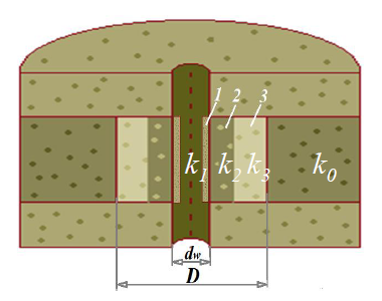
\includegraphics[width=0.6\textwidth]{pic/near-wellbore.png}}
	\caption{Структура ОЗП, образующаяся в результате различных технологических операций. Выделяют:
	\textit{1} -- внешняя фильтрационная корка,
	\textit{2} -- внутренняя корка (зона кольматации), 
	\textit{3} -- зона проникновения фильтрата.}
	\label{pic:near_wellbore}
\end{figure}

	Тем не менее, без особой нужды, при моделировании притока к скважины не рассматривают такую сложную структуру ОЗП. Обычно считают, что вокрук скважины есть кольцевая область с ухудшенной проницаемостью $k_d \leq k$, cм. Рис \ref{pic:near_wellbore_our}.

	При таком подходе скин-фактор $s_d$, отвечающий за повреждение породы, можно найти из выражения:
\begin{equation}
	\label{skin_damage}
	s_d = \left(\frac{k}{k_d}-1\right)\ln\left(\frac{r_d}{r_w}\right).
\end{equation}

\begin{figure}[H]
	\centerline{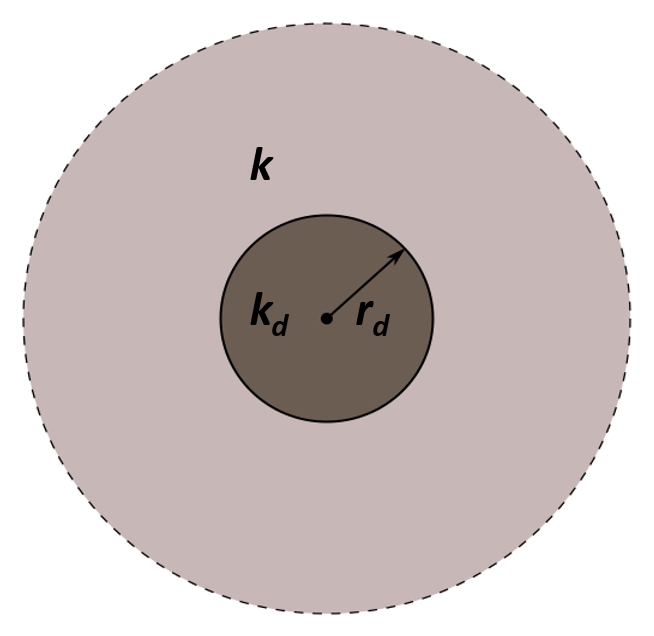
\includegraphics[width=0.4\textwidth]{pic/near-wellbore-our.png}}
	\caption{Рассматриваемая модель ОЗП, обладает ухудшенной проницаемостью $k_d \leq k$.}
	\label{pic:near_wellbore_our}
\end{figure}

\subsubsection{Перфорация}
	В конструкцию большинства скважин входит обсадная колонна, которая цементируется с внешней стороны.  Для вызова притока в такой схеме исользуется \textit{вторичное вскрытие} продуктивных горизонтов. Одним из наиболее распространённых методов вторичного вскрытия является применение кумулятивных зарядов, которые устанавливают по спирали и спускают на глубину.
Результатом их использования являются перфорационные каналы (ПК), которые прошивают обсадную колонну, цемент и часть ОЗП. На Рис. \ref{pic:tunnels} изображена характерная схема ПК на забое скважины.

	В результате в ОЗП, области с наибольшим градиентом давления в пласте, течение существенно отличается от радиального, т.к приток теперь сосредотачивается у боковых поверхностей каналов.

	Тем не менее, для такого типа перфорации, в \cite{tariq} приведены корреляции скин-фактора $s_p$, в зависимости от длины каналов $L_p$, угла фазировки $\theta$, расстояния по глубине между каналами $h$, радиуса перфорационного отверстия $r_p$, могут быть записаны в следующем виде:
\begin{align}
	\label{tunnels_skin}
	s_p &= s_H + s_V + s_{wb}, \\
	s_H &= \ln\left(\frac{r_w}{r_{we}}\right), \quad r_{we} = 
	\begin{cases}
		\frac{L_p}{4}, &\quad \theta = 0,\\
		\alpha_{\theta}(r_w + L_p), &\quad \theta \neq 0,
	\end{cases}\nonumber\\
	s_V &= 10^a\left(\frac{h}{L_p}\sqrt{\frac{k_{xx}}{k_{zz}}}\right)^{b-1}\left(\frac{r_p}{2h}\left(1+\sqrt{\frac{k_{zz}}{k_{xx}}}\right)\right)^b,\nonumber\\
	s_{wb} &= c_1(\theta)\exp\left(c_2(\theta)\frac{r_w}{L_p+r_w}\right),\nonumber
\end{align}
	где корреляции для величин $\alpha_{\theta}$, $a$, $b$, $c_1$, $c_2$ можно найти непосредственно в \cite{tariq}, $k_{xx}$ и $k_{zz}$ -- проницаемости пласта в вертикальном и горизонтальном направлениях.

\begin{figure}[H]
	\centerline{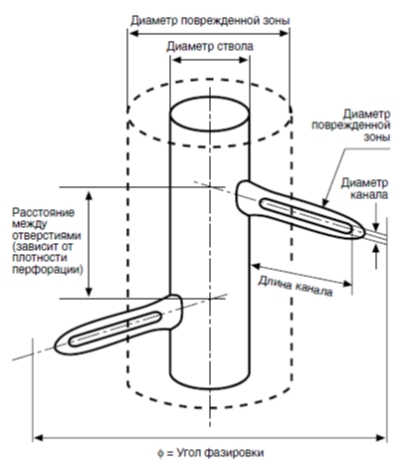
\includegraphics[width=0.6\textwidth]{pic/tunnels.png}}
	\caption{Характерная схема расположения ПК.}
	\label{pic:tunnels}
\end{figure}

	Корреляции \eqref{tunnels_skin} найдены также с использованием явного численного расчёта соответствующих постановок. Ниже будет представлено сравнение численного расчёта, проводимого в текущей работе, постановки с каналами по представленным корреляциям.

\subsubsection{Скважина, несовершенная по степени вскрытия}
	
	С точки зрения терминологии, представленной например в \cite{basniev}, несовершенства скважины разделяют на два типа: скважина несовершенная по \textit{характеру} и \textit{степени} вскрытия. Характер вскрытия был рассмотрен в двух предыдущих пунктах. Степень вскрытия частично рассмотрена в предыдущем пункте. Однако с методологической точки зрения следует рассмотреть отдельно случай частичного проникновения скважины в пласт, неполного его вскрытия.
В данном примере считается что скважина вскрыта в некотором интервале глубин, не содержащим всю мощность пласта, полностью по всему диаметру.

	Впервые выражение для притока к гидродинамически несовершенной по степени вскрытия скважине получил М. Маскет \cite{masket} методом изображений.
	Затем И.А. Чарный \cite{charniy} получил выражение для дополнительного гидродинамического сопротивления:
\begin{align}
	\label{skin_part_penetr}
	s_{pp} &= \left(\frac{1}{\bar{h}}-1\right)\ln\frac{4h}{r_w}-\frac{\phi(\bar{h})}{2\bar{h}}, \\
	\phi(\bar{h}) &= \ln\frac{\Gamma(0.875\bar{h})\Gamma(0.125\bar{h})}{\Gamma(1-0.875\bar{h})\Gamma(1-0.125\bar{h})},\nonumber
\end{align}
	где $\bar{h} = \displaystyle\frac{h_p}{h}$ -- доля вскрытой мощности пласта, $\Gamma(n)$ -- гамма-функция Эйлера.

\begin{figure}[H]

	\begin{subfigure}[b]{0.5\textwidth}
	\centering
	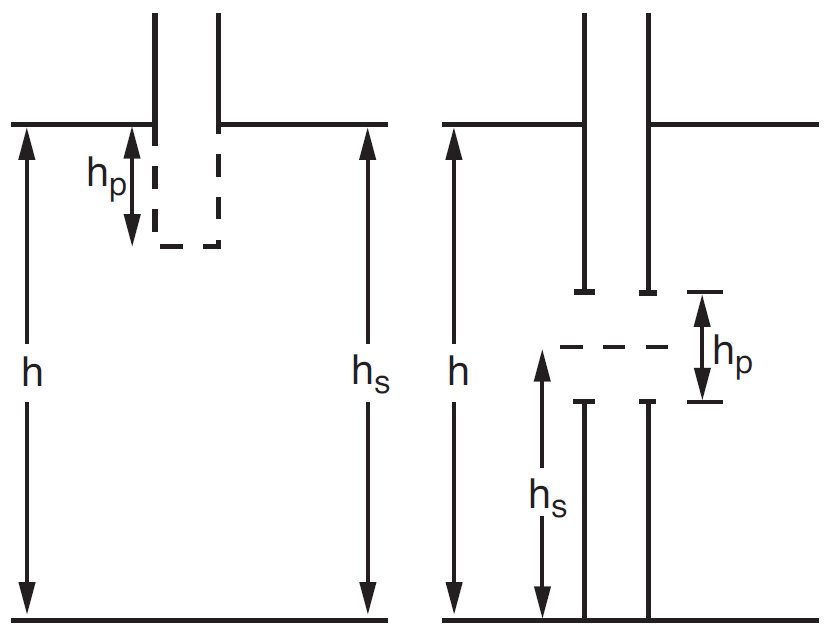
\includegraphics[width=0.5\textwidth]{pic/part_penetrating.png}
	\caption{Скважина с неполным проникновением}
	\label{pic:part_problem}
	\end{subfigure}
~
	\begin{subfigure}[b]{0.5\textwidth}
		\centering
		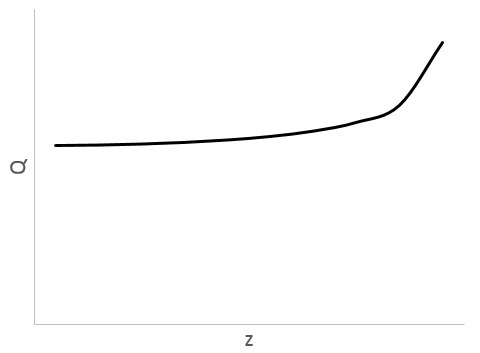
\includegraphics[width=0.7\textwidth]{pic/rate_distr.png}
		\caption{Распределение дебита вдоль ствола}
		\label{pic:rate_distr}
	\end{subfigure}
	\caption{Распределение дебита для несовершенной скважины.}
	\label{pic:part_pen}
\end{figure}

	Отдельным интересным вопросом при расчёте скважины, неполностью вскрывшей пласт (как, впрочем, и каналов), является распределение дебита вдоль перфорированной части. На Рис. \ref{pic:rate_distr} показано установившееся распределение дебита вдоль перфорированной части ствола, при условии постоянства давления вдоль ствола.
Постановка изобрабражена на Рис. \ref{pic:part_problem}.

\subsection{Теплоперенос при фильтрации к несовершенной скважине}
	Выше были рассмотрены основные виды несовршенств скважины, рассматрваемые в данной работе, а также представлены приближённые формулы для расчёта дополнительного гидродинамического сопротивления, возникающего в результате данных несовершенств.
	Подобное рассмотрение возможно лишь в однофазном случае, хотя и для случая многофазной фильтрации некоторые авторы приводят аналитические выражения.
	Рассмотрим влияние этих несовершенств на поведение забойной температуры \cite{ramazanov_spe}.

\subsubsection{Случай совершенной скважины}
	Для начала установим выражение для забойной температуры для притока к совершенной скважине.
	Пренебрегая теплопроводностью запишем уравнение баланса энергии в следующем виде:
\begin{align}
	\label{energy_simple}
	\frac{\partial{T}}{\partial{t}}+u(r, t)\frac{\partial{T}}{\partial{r}} &= -\varepsilon u(r, t)\frac{\partial p}{\partial{r}}
	+\eta^{\ast}\frac{\partial{p}}{\partial{t}}, \\
	u(r, t) = -c\frac{k}{\mu}\frac{\partial{p}}{\partial{r}}, \quad c = \frac{c_o \rho_o}{c_t},  \quad
	c_t &= \phi \rho_o c_o + (1-\phi)\rho_{s}c_s, \quad \eta^{\ast} = \phi c \eta,
\end{align}
	где $u(r, t)$ -- скорость конвективного теплопереноса,
	$\varepsilon$ -- коэффициент Джоуля-Томпсона нефти,
	$\eta$ -- коэффициент адиабатического расширения нефти,
	$c_t$ -- теплоёмкость пористой насыщенной среды.
	
	Уравнение \eqref{energy_simple} учитывает конвективный перенос тепла, а также изменение температуры вследствие 
	\textit{баротермического эффекта}, т.е. изменения температуры вследствие изменения давления.
	По сути баротермический эффект заключает в себе эф-т Джоуля-Томпсона и адиабатическое расширение флюида.
	В уравнении пренебрежено теплопроводностью, т.к. на небольших временах (далее будет уточнено) теплопроводность не даёт существенного вклада в изменение температуры, в сравнение с другими эффектами.

	Замыкая уравнение \eqref{energy_simple} начальным и граничным условиями:
\begin{equation}
	\label{conditions_simple}
	T(r, 0) = T_0, \quad T(r_e, t) = T_0,
\end{equation}
	получим, что \eqref{energy_simple}, \eqref{conditions_simple} -- смешанная задача для гиперболического уравнения в кольце, обладающая аксиальной симметрией.

	Решение задачи \eqref{energy_simple}, \eqref{conditions_simple} можно получить методом характеристик.
	Имеем:
\begin{align}
	\label{sol_simple}
	T(r(t, r_1), t) = T_0 &+ \varepsilon\left[p(r_1, 0)-p(r(t, r_1), t)\right]+
	(\varepsilon+\eta^{\ast})\int\limits_0^t \frac{\partial p(r(\tau, r_1), \tau)}{\partial \tau}d\tau,\\
	\label{chars}
	\frac{dr}{dt}&=u(r, t), \quad r(0)=r_1,
\end{align}

	Далее необходимо найти зависимость $p = p(r, t)$. Примем, для простоты, что флюид и скелет -- несжимаемы, давление устанавливается мнгновенно:
\begin{equation}
	\label{pres}
	p = 
	\begin{cases}
		p_0, &\quad t=0,\\
		p(r), &\quad t>0,
	\end{cases}
\end{equation}
	где $p_0$ -- начальное пластовое давление, $p(r)$ -- стационарное распределение давления:
\begin{equation}
	\label{pres_state}
	p(r) = p_w + \frac{\Delta p \ln\displaystyle\frac{r}{r_w}}{\ln\displaystyle\frac{r_e}{r_w}}
	 = p_w + \frac{Q\mu}{2\pi k h}\ln\frac{r}{r_w},
\end{equation}
	где $\Delta p = p_e - p_w$ -- депрессия на пласт, $Q$ -- объёмный дебит нефти.

	Тогда подставляя \eqref{pres_state} в \eqref{chars}, получим скорость конвективного переноса и уравнение характеристик:
\begin{align}
	\label{convection_speed}
	u(r, t) = -\frac{cQ}{2\pi r h} = -c\frac{k}{\mu}\frac{\Delta p}{\ln\displaystyle\frac{r_e}{r_w}},\\
	\label{chars_sol}
	r = \sqrt{r_1^2 - \displaystyle\frac{cQ}{\pi h}t} = \sqrt{r_1^2 - 2c\displaystyle\frac{k}{\mu}\frac{\Delta p}{\ln\displaystyle\frac{r_e}{r_w}}t}.
\end{align}

	Финальное выражение для забойной температуры получим в виде:
\begin{equation}
	\label{temperature}
		T(r_w, t) = 
	\begin{cases}
		\displaystyle\frac{\varepsilon Q}{2\pi \sigma}\left[\ln\displaystyle\frac{r_T}{r_w}-d\ln\displaystyle\frac{r_e}{r_T}\right] = \displaystyle\frac{\varepsilon \Delta p}{\ln \displaystyle\frac{r_e}{r_w}}\left[\ln\displaystyle\frac{r_T}{r_w}-d\ln\displaystyle\frac{r_e}{r_T}\right], &\quad t\leq t_{st} ,\\
		\varepsilon \Delta p =  \displaystyle\frac{\varepsilon Q}{2\pi\sigma}\ln\frac{r_e}{r_w}, &\quad t>t_{st},
	\end{cases}
\end{equation}
\begin{equation}
	\label{terms33}
	r_T = \sqrt{r_w^2 + \frac{cQ}{\pi h}t}, \quad
	\sigma = \frac{kh}{\mu}, \quad d = \frac{\eta^{\ast}}{\varepsilon}, \quad
	t_{st} = \frac{\pi h r_e^2}{cQ},
\end{equation}
	где $r_T$ имеет смысл радиуса зондирования пласта,
	$\sigma$ -- проводимость,
	$t_{st}$ -- время выхода температуры на стационар.

	Зачастую параметр $d$ мал и член, отвечающий за адиабатику, опускают. Тогда имеем:
\begin{equation}
	\label{temperature1}
	T(r_w, t) = \frac{\varepsilon Q}{4 \pi \sigma}\ln\left[1+\frac{cQ}{\pi h r_w^2}t\right]	\approx
	\frac{\varepsilon Q}{4 \pi \sigma}\left[\ln\frac{cQ}{\pi h r_w^2}+\ln t\right],
\end{equation}
	где правое выражение записано в предположении, что $t \gg \displaystyle\frac{\pi h r_w^2}{cQ}$.
	
	В координатах $(\ln{t}, T)$ зависимость в правой части \eqref{temperature1} будет представлена прямой, коэффициент наклона которой будет обратно пропорционален проводимости $\sigma$.
	Это выражение очень похоже на аналогичное выражение для давления при исследовании ГДИ, для него применимы аналогичные методы интепретации данных.

\subsubsection{Случай несовершенной скважины}
	Тут под несовершенством понимается ухудшенные ФЕС ОЗП, а также перфорацию.
	Суммарный скин-фактор будет равен: $s = s_1 + s_2$, где скин $s_1$ ответственен за перфорацию, а $s_2$ -- за повреждение ОЗП.
	
	Первоначально будет зондирована ОЗП с проводимостью $\sigma_1 = \frac{k_dh}{\mu}$. Скин-фактор при этом будет равен:
	$s = s_1$.
	Соответствующее выражение для температуры имеет вид:
\begin{equation}
	\label{temperature2}
	T(r_w, t) = \frac{\varepsilon Q}{4 \pi \sigma_1}\left[\ln\frac{cQ}{\pi h r_w^2}+\ln t + 2s_1\right],
	\quad r_T < r_d.
\end{equation}
	
	Когда же радиус зондирования превысит размер ОЗП: $r_T \geq r_d$.
	Проводимость будет равна: $\sigma_2 = \frac{kh}{\mu}$, скин -- $s = s_1 + s_2$.
	Для скин-фактора $s_2$ верно выражение \eqref{skin_damage}.
	Выражение для температуры предстанет в виде:
\begin{equation}
	\label{temperature3}
	T(r_w, t) = \frac{\varepsilon Q}{4 \pi \sigma_2}\left[\ln\frac{cQ}{\pi h r_w^2}+\ln t + 2s_1 + 2s_2\right],
	\quad r_T \geq r_d.
\end{equation}

	В коодинатах $(\ln{t}, T)$ выражения \eqref{temperature2}, \eqref{temperature3} будут иметь вид прямой:
\begin{align}	
	\label{imperfect_lines}
	T &= A + B\ln t,\\
	A_1 &= B_1\left[\ln\frac{cQ}{\pi h r_w^2} + 2s_1\right], \quad B_1 = \frac{\varepsilon Q}{4\pi\sigma_1},\\
	A_2 &= B_2\left[\frac{A_1}{B_1} + 2s_2\right], \quad B_2 = \frac{\varepsilon Q}{4\pi\sigma_2},\\
\end{align}
	Прямые изображены на Рис. \ref{pic:imperfect_lines}:
\begin{figure}[H]
	\centerline{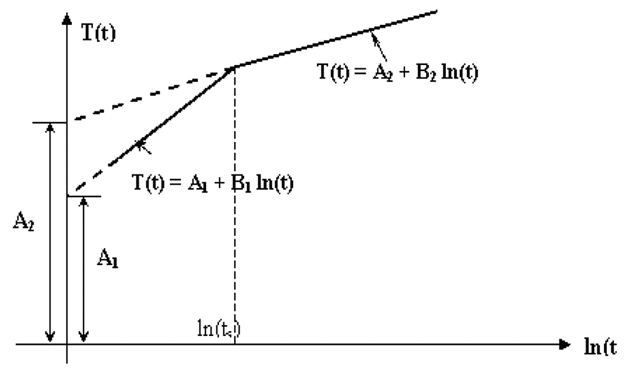
\includegraphics[width=0.6\textwidth]{pic/imperfect_lines.png}}
	\caption{График для забойной температуры в осях $(\ln t, T)$. Первый участок соответствует зондированию ОЗП, второй -- зондированию пласта.}
	\label{pic:imperfect_lines}
\end{figure}

	Результатом этого рассмотрения является нахождение проницаемостей $k_d$, $k$ ОЗП и пласта и скин-факторов $s_1$, $s_2$, ответственных за перфорацию и повреждение ОЗП, из графика забойной температуры при выходе на режим. Этот метод носит название -- \textit{метод термозондирования Э.Б. Чекалюка} \cite{checkalyuk}.

	Тут стоит отметить, что метод имеет существенные ограничения по применению. Во-первых, метод рассматривает лишь однофазную фильтрацию. Во-вторых, характерное время когда $r_T = r_d$ составляет несколько часов. Этот период времени, часто лежит в области эффекта влияния ствола скважины (ВСС), который может существенно повлиять на динамику температуры, особенно когда датчик находится на некотором удалении от забоя скважины. Поэтому метод может быть использован лишь в ограниченном круге примеров, в качестве первого приближения.
	
	На Рис. \ref{pic:analytic_cmp} представлено сравнение аналитики \eqref{temperature1}, \eqref{imperfect_lines} с численным расчётом:
	
\begin{figure}[H]

	\begin{subfigure}[b]{0.5\textwidth}
		\centering
		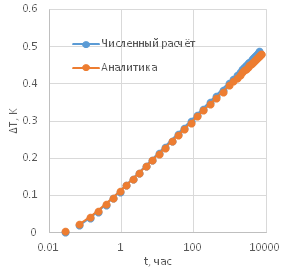
\includegraphics[width=0.9\textwidth]{pic/perfect.png}
		\caption{Совершенная скважина}
		\label{pic:perf}
	\end{subfigure}
~
	\begin{subfigure}[b]{0.5\textwidth}
		\centering
		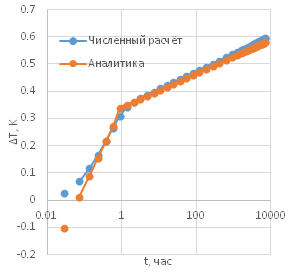
\includegraphics[width=0.9\textwidth]{pic/imperf1.png}
		\caption{Несовершенная скважина с параметрами: $s_2=5, r_d = 0.2$}
		\label{pic:imperf1}
	\end{subfigure}
	\begin{subfigure}[b]{0.5\textwidth}
		\centering
		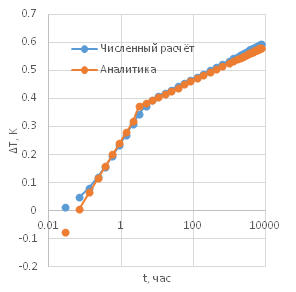
\includegraphics[width=0.9\textwidth]{pic/imperf2.png}
		\caption{Несовершенная скважина с параметрами: $s_2=5, r_d = 0.4$}
		\label{pic:imperf2}
	\end{subfigure}
~
	\begin{subfigure}[b]{0.5\textwidth}
		\centering
		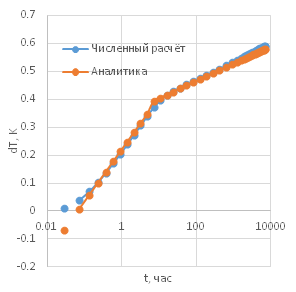
\includegraphics[width=0.9\textwidth]{pic/imperf3.png}
		\caption{Несовершенная скважина с параметрами: $s_2=5, r_d = 0.6$}
		\label{pic:imperf3}
	\end{subfigure}
	\caption{Сравнение аналитического и численного расчёта для совершенной и несовершенной скважины при различных размеров ОЗП.}
	\label{pic:analytic_cmp}
\end{figure}
